\PassOptionsToPackage{unicode}{hyperref}
\PassOptionsToPackage{hyphens}{url}
%

\documentclass[12pt, a4paper]{article}
\usepackage[a4paper,margin=1in]{geometry}
\setlength\parindent{0pt}
\usepackage{mathptmx}
\usepackage{amsmath,amssymb}
\usepackage[T1]{fontenc}
\usepackage[utf8]{inputenc}
\usepackage{textcomp}
\usepackage{pgfplots}
\usepackage{verbatim}
\usepackage{hyperref}
\usepackage{graphicx}
\usepackage{placeins}
\graphicspath{{img-tables/}}

\author{Mattia Buzzoni, Artificial Intelligence Master Degree, ID number 0001145667
\\Leonardo Mannini, Artificial Intelligence Master Degree, ID number 0001135209
\\Mirko Mornelli, Artificial Intelligence Master Degree, ID number 0001113084
\\Riccardo Romeo, Artificial Intelligence Master Degree, ID number 0001145681
\\Diego Rossi, Artificial Intelligence Master Degree, ID number 0001138652}
\date{05-23-2025}
\title{A Song of Ice and Fire}

\begin{document}
	\maketitle
	
	\section{Introduction}
	\label{introduction}
	The analysis of narrative structures is a wide field that shows the complexity of human society and imagination. A specific area, narrative fiction, especially epic fantasy, is a good source for analyzing structures and characters. The series A Song of Ice and Fire by George R. R. Martin is a very complex example of modern fantasy. Its large number of characters, changing alliances, and complex plots make it an interesting topic for both literary and computational study.
	This project is part of digital literary studies, combining narrative analysis and network science. We focus on the social structures in A Song of Ice and Fire, looking at character interactions in the five published books. These books describe a growing universe with hundreds of characters, each playing a part in a large political and personal story.
	
	To understand the structure of these character interactions, we use  Network Analysis. This lets us represent the story as a graph, where characters are nodes and their interactions are edges. By studying these networks with computational tools, we want to get quantitative information about the story's structure. Specifically, we look at how character importance, community structures, and connections change across the five books.
	
	
	\section{Problem and Motivation}
	\label{problem-and-motivation}
	
	This project investigates the character interaction structures in the first five books of \textit{A Song of Ice and Fire}. The central aim is to explore characters' social positioning and assess their evolving importance in a saga characterized by a complex, distributed cast whose relevance shifts over time and context.

	The core problem is identifying and evaluating character centrality within this fragmented, multi-perspective narrative. Determining key figures and their influence in a universe of hundreds of characters with diverse alliances and roles presents a significant narrative and analytical challenge. 
	
	The project's main contribution is mapping and analyzing the evolving character interaction network across the five books. This highlights patterns of centrality, influence, and group formation, aiming to illuminate epic fantasy's storytelling mechanisms and demonstrate how network analysis can enrich our understanding of literary worlds.
	\section{Datasets}
	\label{datasets}
	
	The character network for Game of Thrones (the A Song of Ice and Fire novels) comes from a dataset available to the public. 
	This dataset creates connections (edges) between characters based on when their names appear close to each other in the text. 
	
	Specifically, an edge is made if two characters' names are within 15 words of each other in the books. 
	This method can be used as a good way to know if characters are in the same scene, talk to each other, or are mentioned together. 
	
	The 15-word window is meant to be small enough to show a direct connection but large enough to catch most immediate interactions. Any window size can seem a bit random and might not perfectly catch every detail of interactions (for example, quick mentions could be missed, or names that are not related but appear in a crowded part of the text might be linked). However, it gives a consistent way to define interactions from the text that others can repeat. Basically, a link in the network means there's a contextual relationship. This could mean that two characters talked to each other, talked about each other, or were mentioned together. The strength of a connection (its weight) is the number of times these co-occurrences (interactions) happen between two characters. 
	
	The dataset has CSV files (one for each book) that list pairs of character names and how many times they co-occur. Using this data, we built an undirected, weighted graph for each of the five books, and also a combined network for all books. Each character is a node, and an edge between two nodes means those characters were mentioned near each other in the text. The weight on each edge shows how many times the characters appear together. This acts as a measure of how strong their relationship is in the story (for example, characters who meet or talk often will likely have a higher weight).
	
	
	\subsection*{Data Collection and Pre-processing}
	
	The character-co-occurrence edge lists we analyse come from a community dataset on Kaggle entitled Game of Thrones Network.
	The dataset's author parsed the full text of the five published novels and recorded every pair of character names that occur within a 15-word sliding window.
	
	In our own notebook, we performed only light additional cleaning. 
	The combined graph has 796 nodes and 2 823 weighted edges.
	
	\subsection*{Tools Used}
	We used Python and its libraries for all data processing and analysis. Specifically, we used pandas for handling data and NetworkX for creating graphs and doing network analysis. We used other packages like Matplotlib for plotting.  All our code and processed data are available in a public GitHub repository.
	\section{Validity and Reliability}
	
	\label{validity-and-reliability}
	Because the dataset came from a user on Kaggle and not from official text notes, the data might not be perfectly accurate. Possible problems include missed co-occurrences, wrong edges, or names that are not consistent. Even with these issues, the dataset seems to be quite valid because its patterns match the known story of the books well. In fact, one of our goals was to check the dataset by seeing if known story structures appeared in the network analysis. 
	
	More than just qualitative checks, the dataset's reliability is supported by the fact that it can be reproduced and is consistent with other studies. This means anyone could create the co-occurrence network again from the original text and would 
	likely get a very similar list of connections. 
	
	
	For internal consistency, we made sure to do the analysis the same way for each book, we used the same metrics and algorithms 
	for all five networks, with the same settings, so comparisons between books should be valid. In short, even if the dataset isn't perfect, 
	the evidence shows it's accurate enough for a useful analysis: the network patterns that appear seem to reflect the Game of Thrones story, 
	and the method can be repeated. 
	
	The results show a clear consistency with the "A Song Of Ice And Fire" story, which makes us more confident that the dataset is valid and also reliable, together with the documentation of the dataset which was collected and processed in a meaningful way.
	
	
	
	\section{Measures and Results}
	\label{measures}
	To measure the roles and importance of characters in the network, we calculated several centrality measures and other graph metrics. Each of these measures shows a different side of a character's importance or position in the social network. Below, we will briefly explain each metric and then talk about what we found for each book and for the whole series.
	
	\subsection*{Degree Centrality}
	Degree centrality, 
	is the number of edges each node has. 
	A high degree means the character interacts with or is
	mentioned with many others, making them a center of the network. 

	This measure naturally shows a character's
	visibility and direct involvement in the story. 
	In our study, Tyrion Lannister has the highest 
	degree centrality in all five books. 
	Degree centrality gives a basic ranking of characters 
	by how connected they are, but it doesn't look at who 
	they are connected to.
	
	\begin{figure}[htbp]
		\centering
		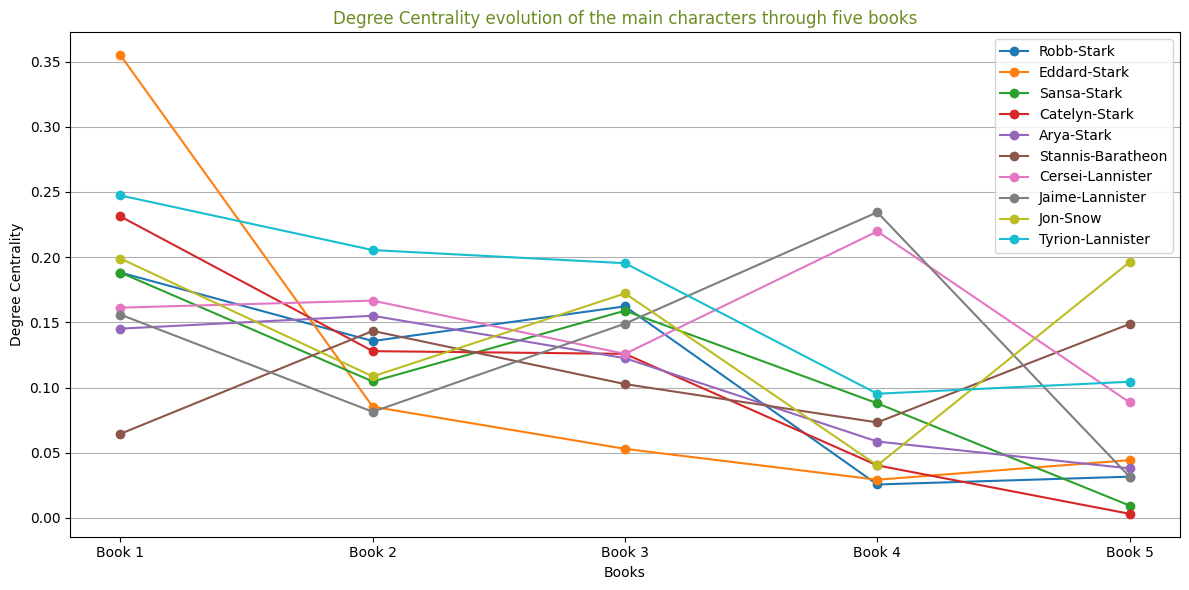
\includegraphics[width=0.8\textwidth]{deg-cent-evolution.png}
		\caption{Degree Centrality evolution of the main characters through five books.}
		\label{fig:deg_cent_evolution}
	\end{figure}
	\FloatBarrier
	\subsection*{Eigenvector Centrality}
	Eigenvector centrality identifies important characters by their connections to other important people. Histograms consistently show extreme skewness: most characters have values <1, while a few reach very high scores. The cumulative curve, initially slow, rises sharply at these ``elite'' nodes, a pattern intensifying in later books. The combined network's distribution, spanning two orders of magnitude, confirms the saga's plot revolves around a small group of ``star'' characters whose prestige radiates throughout.

	Intuitively, high-status figures (e.g., Robert, Cersei, Daenerys) connected to other influential individuals have explosive eigenvector scores, while minor characters interacting with other marginal figures maintain tiny values. This pyramidal structure means the distribution isn't strictly scale-free (power law exponent not between 2-3). However, a long heavy tail and log-log linear segments in cumulative plots indicate underlying power-law mechanisms: prominent characters gain further prominence, while the narrative focuses on them amidst many transient, low-impact side characters.

	\subsection*{Katz Centrality}
	Katz centrality is an extension of eigenvector centrality:
	every character starts with a small baseline score and then
	gains additional influence from walks of length two, three, 
	and so on, each step counting a little less than the previous one. 
	
	
	When we compute the measure on the full five-book network, 
	Tyrion Lannister emerges as the first one,
	with Jon Snow in a close second place. 
	Immediately behind them come Jaime Lannister, 
	Cersei Lannister, and Stannis Baratheon. Jon's score climbs book 
	after book, reflecting how his storyline gradually connects the 
	Night's Watch, the wildlings, the northern houses, and even the 
	Iron Throne via correspondence. 
	
	This metric  reinforces what simpler measures already indicated, 
	Tyrion and Jon dominate the narrative, but it adds something. 
	It shows Jon's influence catching up over time and highlights 
	characters such as Stannis and Arya, who do not have the 
	highest degree counts yet serve as effective conduits that
	link otherwise distant parts of the network.
	
	
	\subsection*{Closeness Centrality}
	Closeness centrality measures how close a character is to all 
	other characters in the network, based on graph distance. 
	Officially, it's the inverse of the average shortest path length 
	from one node to all other nodes. A character with high closeness 
	centrality can reach every other character through just a few steps 
	on average. 
	We found that characters like Tyrion and 
	Cersei Lannister often had some of the shortest average 
	distances to others. Tyrion interacts with 
	many groups. Cersei is in a central place in King's Landing 
	and interacts with various people, so she's never far from any storyline. 
	Interestingly, Petyr Baelish also had a 
	fairly high closeness centrality in the early books even if it is a secondary character,
	making him an almost universal 
	connector in the network. So, closeness centrality 
	highlighted characters who act as hubs connecting 
	communities.
	
	\subsection*{Betweenness Centrality}
	Betweenness centrality measures how often a node is on the 
	shortest path between any two other nodes. It effectively 
	finds the ``bridge'' characters in the network, those who 
	connect different communities or whose presence is key for 
	information to flow in the network. A character with high 
	betweenness centrality might not have the most connections, 
	but they are at important points between storylines. 
	
      Our betweenness analysis gave some of the most interesting 
	results, as it pointed out a few characters we didn't expect. 
	If you ``remove'' these characters and their connecting nodes, 
	the network splits, their followers 
	and their interactions with other groups would be cut off. 
	So, these characters act as  vital links between otherwise separate 
	groups. 
	
	
	Betweenness centrality also
	showed which characters might act as bridges in the story. It's 
	worth noting that betweenness didn't always match perceived plot 
	importance. Some very central characters by other measures 
	have storylines that are fairly separate, 
	so they don't score high on betweenness 
	because they don't act as links between different groups. 
	On the other hand, characters who move between groups 
	can have high betweenness. 
	
	\begin{figure}[htbp]
		\centering
		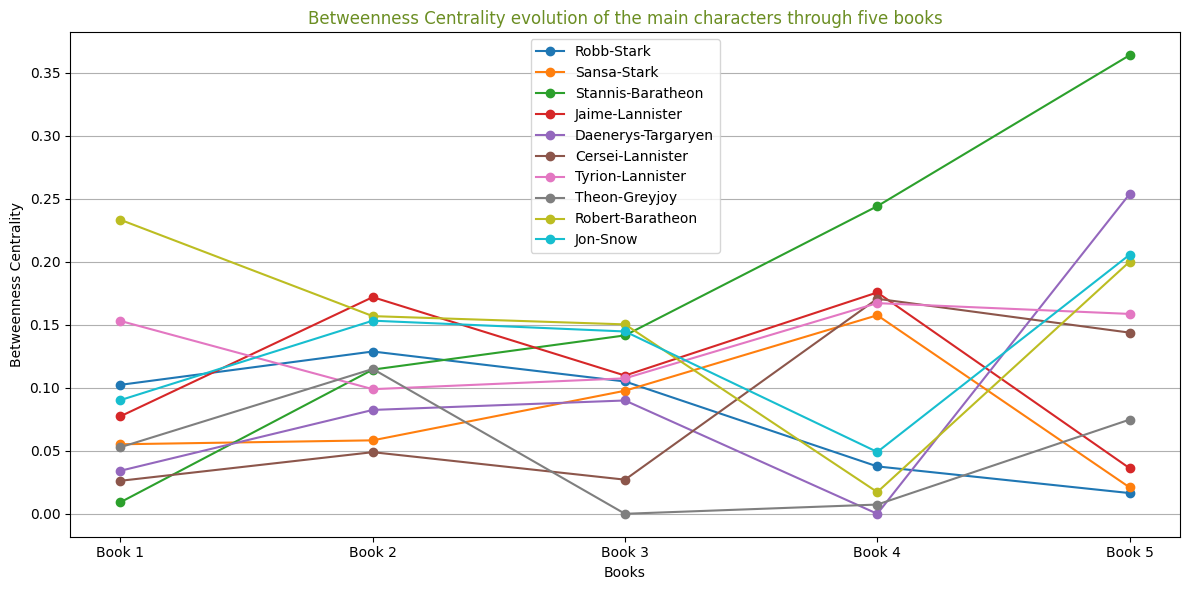
\includegraphics[width=0.7\textwidth]{betweenness-all.png}
		\label{fig:betweennessall}
	\end{figure}
	\FloatBarrier
	
	
	\subsection*{Cliques}
	We identified all cliques in each book's network. The largest cliques
       occur in the earlier books, where the narrative brings many main 
       characters together. For example, in Book 1 one of the largest 
       cliques included characters corresponding to the gathering of 
       major figures at the King's Landing. We also found family-based
        cliques. Notably, the Stark family form a clique in Book 1. 
        In later books, cliques tend to be smaller as the story splits 
        geographically. This shows the data correctly captures close 
        groups – whenever a set of characters all interact heavily, 
        it appears as a clique, often aligning with narrative events 
        like councils, feasts or family meetings. 
	We focused on the largest cliques (of size greather than 3) 
      and meaningful ones (like family cliques), since a great many 
      trivial small cliques (triangles) exist. What cliques reveal 
      is the community structure at its most strict definition: they 
      highlight factions or scenes where everyone knows everyone else. 
	
	A clique requires every possible edge to be present, 
      which is a strong condition. 
      Thus, many cohesive groups in the story won't appear as a full clique. 
      We mitigated this by also examining k-cores and other measures for 
      group cohesion. Clique analysis confirmed that the network 
      representation picks up known "close" groups.
	
	\begin{figure}[htbp]
		\centering
		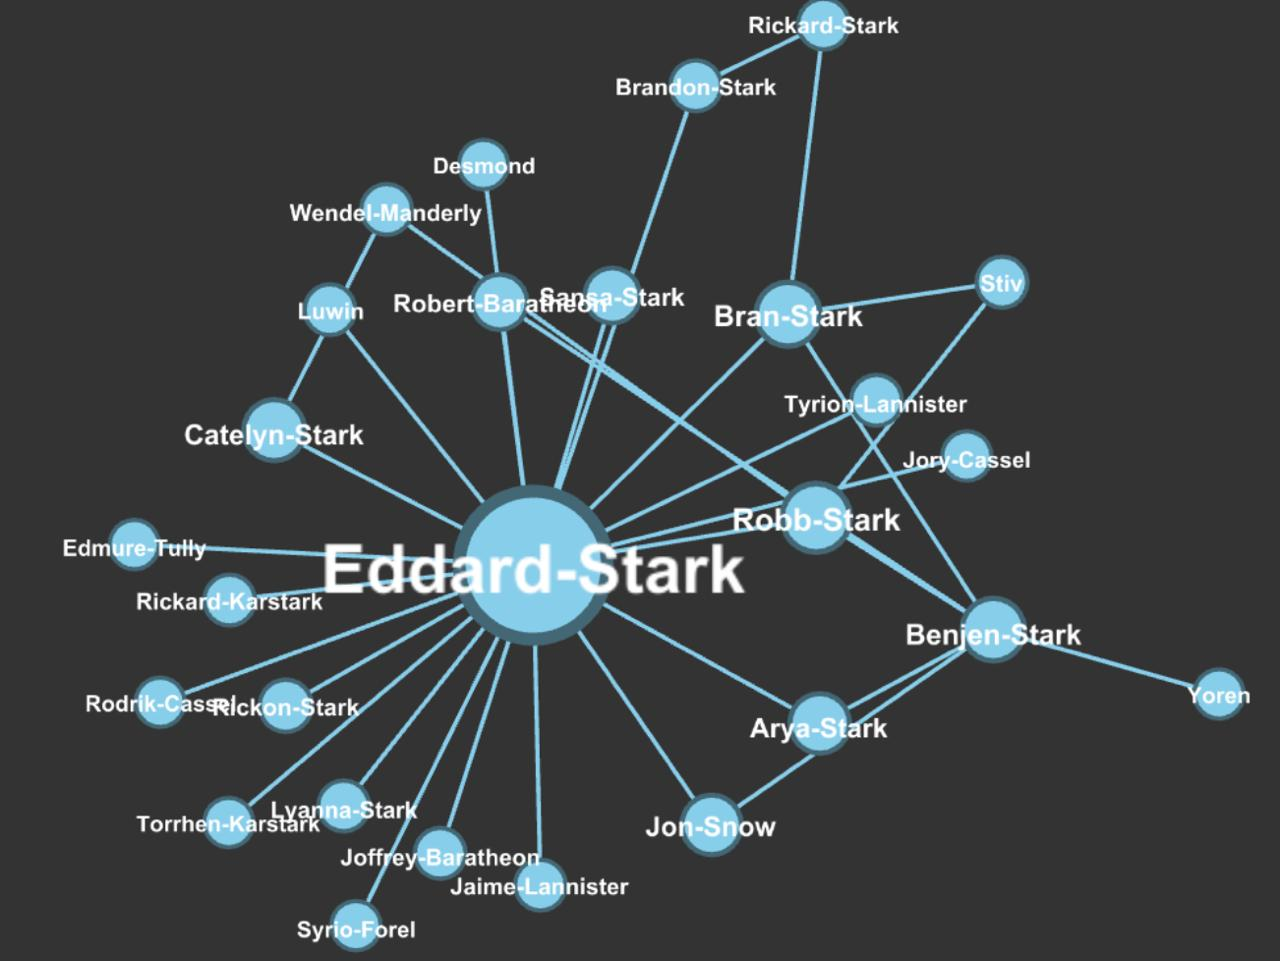
\includegraphics[width=0.7\textwidth]{clique_stark.jpeg}
		\label{fig:cliquestark}
            \caption{Clique of the Stark family in Book 1.}
	\end{figure}
	\FloatBarrier
	
	\subsection*{K-cores}
	
	We performed a core decomposition to find k-cores. 
      In each book, we found a clear highest-order core. 
      In Book 1 and Book 2, the highest core was of order 11: 
      By Book 3, the maximum core was slightly lower, and 
      it drops further in Book 4 and 5 (e.g. only a 7-core in Book 4). 
      This trend quantifies the narrative's structural change: 
      Book 1-2 have a very interconnected core cast, whereas later books fragment 
      the cast, so you cannot find as large a group all mutually connected. 
	
	We found that the composition of the high-order cores aligns with 
      major story factions.
	
	K-cores give a layered view of network density. 
      The highest k-core in each book essentially isolates the most central 
      group of characters. We observed that these tend to be centered 
      on political power hubs (court, major families). As k decreases, 
      cores grow larger, bringing in progressively less-connected characters. 
      It shows that the books have a relatively small inner-core driving interactions 
       (often <20 characters).

	In general, K-core analysis supported that our network data 
      is story-consistent: e.g. the cores we found contained coherent 
      sets of characters, reinforcing that interactions were correctly identified.
	\begin{figure}[htbp]
		\centering
		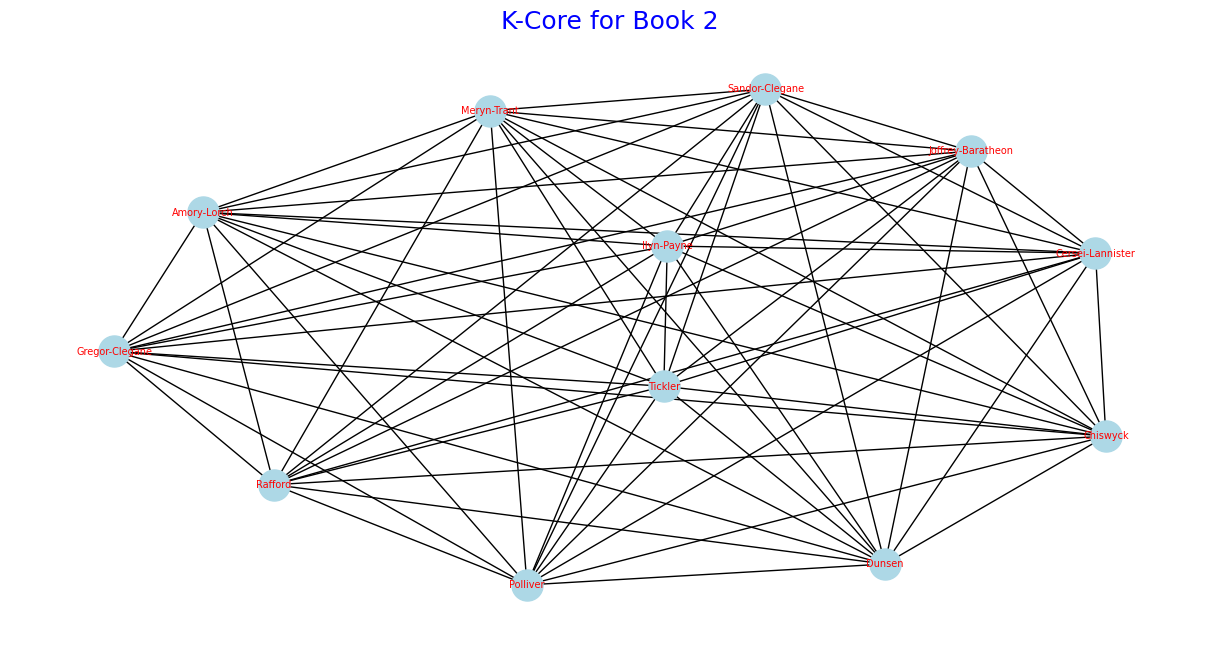
\includegraphics[width=0.8\textwidth]{k-core-book2.png}
		\caption{K-core of a network of Book 2.}
		\label{fig:kcore}
	\end{figure}
	\FloatBarrier
	\subsection*{K-components}
	
	We analyzed k-components, which relate to the network's structural cohesion.
	
	The story networks exhibited many small 2-components,
       but no giant 2-component containing all main characters.
        This indicates that the network has articulation points, 
        characters whose removal would break apart the graph. 
	We saw that most higher k-components were tiny groups of 
      characters who form a fully interconnected cluster. 
	
	For example, Arya Stark in Book 4 forms a 2-component with 
      two of her Braavos contacts ("Waif" and the Kindly Man): 
      Arya interacts with each of them and they interact 
      (as teacher and fellow acolyte), making a triangle. 
      One significant 2-component in Book 5 was Bran Stark's 
      cohort beyond the Wall, forming a biconnected group; 
      they are all in the same storyline, and they have multiple 
      paths of interaction. 
	
	The presence of such 2-components indicates pockets of 
      the narrative that are very cohesive. 
	
	The lack of a large 2-component including all major 
      characters means the narrative has key "single points 
      of failure". Indeed, if you "remove" certain central 
      characters (for example, Tyrion Lannister in the early books), 
      many others would lose their only connection and the network 
      would fall into components. In fact, our analysis showed that 
      the main giant component of each book is held together in 
      part by a few critical connectors (which ties in with our 
      betweenness findings). The small higher-order components 
      we found (triads, small cliques) correspond to tightly-knit 
      subgroups – typically members of the same family or people 
      jointly involved in a particular subplot.
	
	Our k-component analysis simply confirmed that, beyond 
      the obvious cliques, the network contains no larger 
      redundant sub-structures. Overall, the story graph 
      is essentially tree-like: many branches extend from 
      just a few trunk nodes. In practice, focusing on 
      2-components was enough, as we found no non-trivial 
      3-components.
	

	
	\subsection*{Local Clustering Coefficient}
	For each character, we calculated their local clustering coefficient.
	
	We observed a wide range of LCC values, strongly correlated on a character's role. Major bridging characters had low clustering, whereas characters embedded in a single group had high clustering. 
	
	In general, we found that characters who only appear within one close setting (e.g., members of the same household) often had very high clustering coefficients. In contrast, characters who serve as go-betweens connecting different groups had low LCC because those sets of neighbors don't interact with each other. 
	
	We also looked at the average clustering: Book 1's average clustering coefficient was relatively higher than later books. This is intuitive since Book 1's main characters largely interact in one location (yielding interconnected neighbor sets). In later books, many characters have neighbors spread across disparate locales who never meet each other, lowering clustering. 
	
	One  consideration is that, our co-occurrence network might count characters as "neighbors" if they are merely mentioned in the same chapter, even if they don't form a meaningful social tie.
	
	\subsection*{Structural Equivalence} 
	We examined how similar characters are in terms of whom they interact with. To compute this, we used metrics like the Jaccard coefficient, Pearson correlation, and Hamming distance. 
	
	We found that perfect structural equivalence was rare. However, in Book 2, a trio of historical Targaryen princes (Aegon V, Daeron II, and Maekar I) are mentioned exclusively together in one anecdote; all three have the same neighbors, so any pair of them is structurally equivalent. 
	The analysis didn't show any pair of major independent characters being extremely similar – which makes sense, since each protagonist has a unique journey. 
	
	One caveat is that our similarity analysis rests on co-occurrence data, which can blur narrative roles. Two characters may appear in every scene together simply because they travel side by side, not because they serve the same plot function. Pearson correlation is also sensitive to differences in degree, so we used it mainly to validate what Jaccard revealed or to catch cases Jaccard missed.
	
	We found that the top-ranked similarities were straightforward to interpret—mostly obvious co-travelers.
	
	\subsection*{Jaccard Coefficient}
	
	To measure how much two characters' social circles overlap, we computed the
	Jaccard coefficient for every pair of nodes.
	
	The very few pairs that reach the maximum value of 1.0 are almost always
	walk-on figures who appear together in a single scene or locale—for example,
	\textit{Robert Arryn–Trystane Martell}, both merely mentioned in one small
	council meeting in Book 2.  Because these cameo characters are seen only in the
	company of the same handful of protagonists, they inherit identical
	neighbourhoods and are effectively interchangeable background.
	
	Conversely, pairs with a coefficient of 0.0—such as \textit{Addam Marbrand}
	versus almost any peripheral Night's Watch ranger—belong to storylines that
	never intersect.  The large volume of zero-overlap pairs quantifies the
	saga's strong modularity: until later books, characters rooted in King's
	Landing politics have no common neighbours with those beyond the Wall or in
	Essos.
	
	Taken together, the distribution of Jaccard values reveals two key features
	of the network.  First, extremely high scores cluster on peripheral nodes,
	confirming that cameo characters are weakly embedded and gain their few links
	solely from co-occurring with a single protagonist.  Second, the abundance of
	zero scores maps the sharp boundaries between parallel narrative communities.
	
	\subsection*{Pearson Correlation}
	
	In our network the rare pairs that reach \(+1\) are almost always
	walk-on figures who surface only alongside the same major characters.  
	They serve as interchangeable background and never forge ties of their own.
	
	At the other extreme, strongly negative—or near-zero—correlations arise
	between protagonists such as Tyrion, Jon, Daenerys and Catelyn.
	These leading characters act in storylines that are geographically and
	socially isolated, each assembling a distinct entourage.
	
	Thus, Pearson correlation does not underlie any important information with respect to the Jaccard Coefficient.
	
	\subsection*{Hamming Distance}
	
	Computing the Hamming Distance, we see that the biggest distances are almost always between main characters who live in separate story lines.
	In Book 1 the pair "Eddard – Daenerys" has a huge distance.
	Later books show the same pattern: Tyrion vs Jon, or Daenerys vs Stannis, get the top scores because each one moves with a unique group of allies and enemies.
	
	On the opposite side, walk-on characters that appear together in the same single scene get a distance of zero.
	
	
	So, the Hamming Distance confirms what we have found previously.
	
	
	\subsection*{Regular Equivalence}
	
	Our regular-equivalence analysis shows that each novel in A Song of Ice and Fire re-deploys a small set of structural templates—kings and queens, counsellors, heirs, and pretenders—even as the action shifts across continents.
	
	\begin{itemize}
		\item Book 1. The strongest equivalence links Eddard Stark and Robert Baratheon. Cersei Lannister scores next, her place in the royal triangle making her structurally close to both Eddard and Robert.
		\item Book 2. Tyrion and Joffrey emerge as the most equivalent pair: Tyrion rules as Acting Hand while Joffrey wears the crown, so they interact with virtually the same courtiers and guards.
		\item Book 4. Leadership is recast as a triad of Cersei, Tommen, and Margaery. The child-king and the two rival queens are tightly coupled to one another and to the shared Lannister–Tyrell power web.
		\item Book 5. The same royal pattern is transplanted to Meereen. At the centre stands Daenerys, whose closest equivalents are Hizdahr and Barristan. Quentyn, Daario.
	\end{itemize}
	
	These patterns show that, even when the plot moves across continents, the social graph keeps re-using a limited set of structural templates—kings and queens, counsellors, heirs, pretenders-and regular equivalence is able to detect those templates automatically.
	
	\subsection*{Homophily – Assortative Mixing}
	
	Homophily is measured through the \emph{degree assortativity coefficient}, the Pearson correlation between the degrees of the two nodes at every edge.  
	Across the five novels the coefficients are
	\[
	-0.166,\;-0.125,\;-0.133,\;-0.137,\;-0.185,
	\]
	and the aggregate network yields \(-0.133\).

	All coefficients are negative, indicating a disassortative structure where high-degree ``hub'' characters tend to connect with low-degree ``peripheral'' ones rather than with each other. Each protagonist forms a local star: a central figure surrounded by minor characters who seldom interact among themselves—faithful to the vast, hierarchical world of Westeros.

	The evolution across books highlights this trend. Book 2, with a coefficient of \(-0.125\), shows the weakest disassortativity. Here, action is still clustered in King's Landing, many characters share similar numbers of contacts, and the graph is less star-shaped. In contrast, Book 5 exhibits the strongest disassortativity (\(-0.185\)).
  

	In short, the increasingly negative assortativity quantifies the saga's hierarchical social fabric: a handful of hubs mediate most interactions, and that hierarchy grows sharper as the plot spreads across continents.
	\subsection*{Small-World Effect} 
	
	All our character networks satisfy the classical "small-world'' condition.
	For every book we computed the two standard indicators, 
	$\sigma$ and $\omega$.
	A graph is considered small-world when $\sigma>1$ or, equivalently, when $\omega$ is close to zero.
	Book 1 already meets the requirement with $\sigma=1.64$ and $\omega=-0.07$, and the effect grows stronger through the series: $\sigma$ rises from $2.21$ in Book 2 to $2.81$ in Book 5, while $\omega$ stays in the narrow band $[-0.19,-0.07]$.
	The aggregated five-book graph shows the same pattern, $\sigma=2.31$ and $\omega=-0.07$.
	
	In practice this means that the story world is highly clustered families, 
	courts and war camps produce many local triangles but, at the same time, 
	any two characters are separated by only a few steps. 
	Bridging figures such as Varys, Littlefinger, 
	Tyrion or, later, Jon Snow and Daenerys act as 
	shortcuts that link distant communities, keeping the average path length almost as low 
	as in a random graph.  The monotonic increase of $\sigma$ from Book 1 to Book 5 reflects
	the geographic expansion of the plot: clustering grows because each new region adds its
	own dense sub-cast, yet the presence of travelling protagonists and frequent cross-mentions
	prevents the network from fragmenting, so the overall structure remains a textbook small world.
	
	
	\subsection*{Degree Centrality} 
	Log-log plots of degree centrality reveal a long tail: few "star" characters (e.g., Tyrion, Daenerys, Eddard) have many connections, while most have few. Fitting this tail to a power law yielded an exponent $\alpha$ outside the 2-3 range, indicating decay steeper than classical scale-free networks. Thus, the story graph has prominent hubs, making it vulnerable to random failure; removing a hub could disconnect numerous sub-plots, as minor characters typically orbit a few protagonists.
	\begin{figure}[htbp]
		\centering
		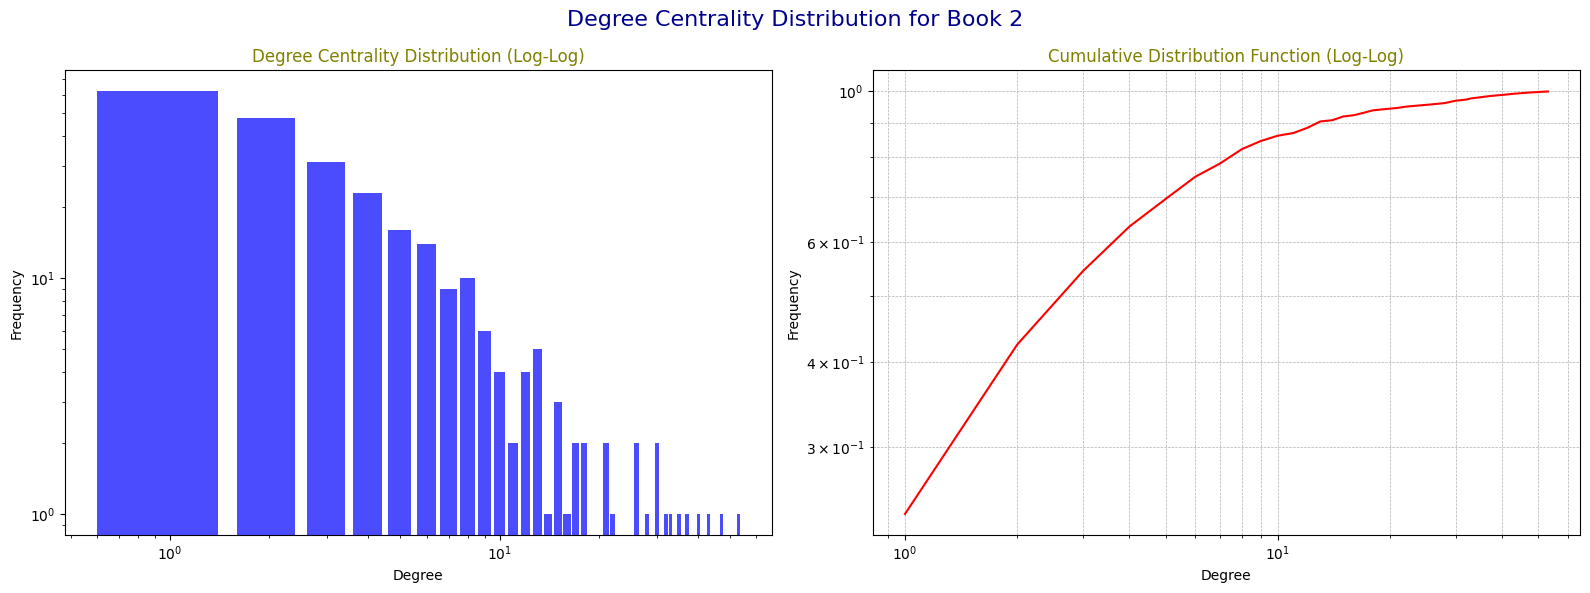
\includegraphics[width=0.8\textwidth]{deg-cent-log-book-2.png}
		\caption{Degree Centrality Distribution for Book 2. Left: Log-log histogram showing a long right tail (few high-degree characters, most with 1-2 links). Right: Cumulative curve indicating a small core concentrates ties, with ~90\% of nodes in the periphery (below degree ten).}
		\label{fig:degcentbook2}
	\end{figure}
      \FloatBarrier
	
	
	\subsection*{Closeness Centrality}
	Closeness looks at distance: a character has high closeness if,
	on average, she can reach every other node through only a few narrative "hops".
	
	
	The histograms are bell shaped instead of heavy-tailed: most characters share a similar, medium closeness, while only a handful sit markedly closer to everyone else.  Those peaks correspond to the obvious hubs of the story, Eddard in \emph{Book1}, Tyrion in \emph{Book2-3}, Cersei in \emph{Book4}, and Daenerys plus Jon in \emph{Book5}.
	From \emph{Book1} to \emph{Book5} the centre of the distribution drifts a little to the right, meaning that the typical distance among nodes becomes shorter: even if the cast grows, the narrative keeps adding shortcuts (for instance the war councils in the North and the royal courts in Meereen) that glue the network together.
	When we put all books in a single graph the curve stretches further, 
	yet the cumulative function on the right panel still reaches $F(x)\approx1$ 
	very quickly; this tells us that the saga preserves a strong "small-village" feeling: 
	information and conflict can spread almost everywhere in  few moves.
	
	\begin{figure}[htbp]
		\centering
		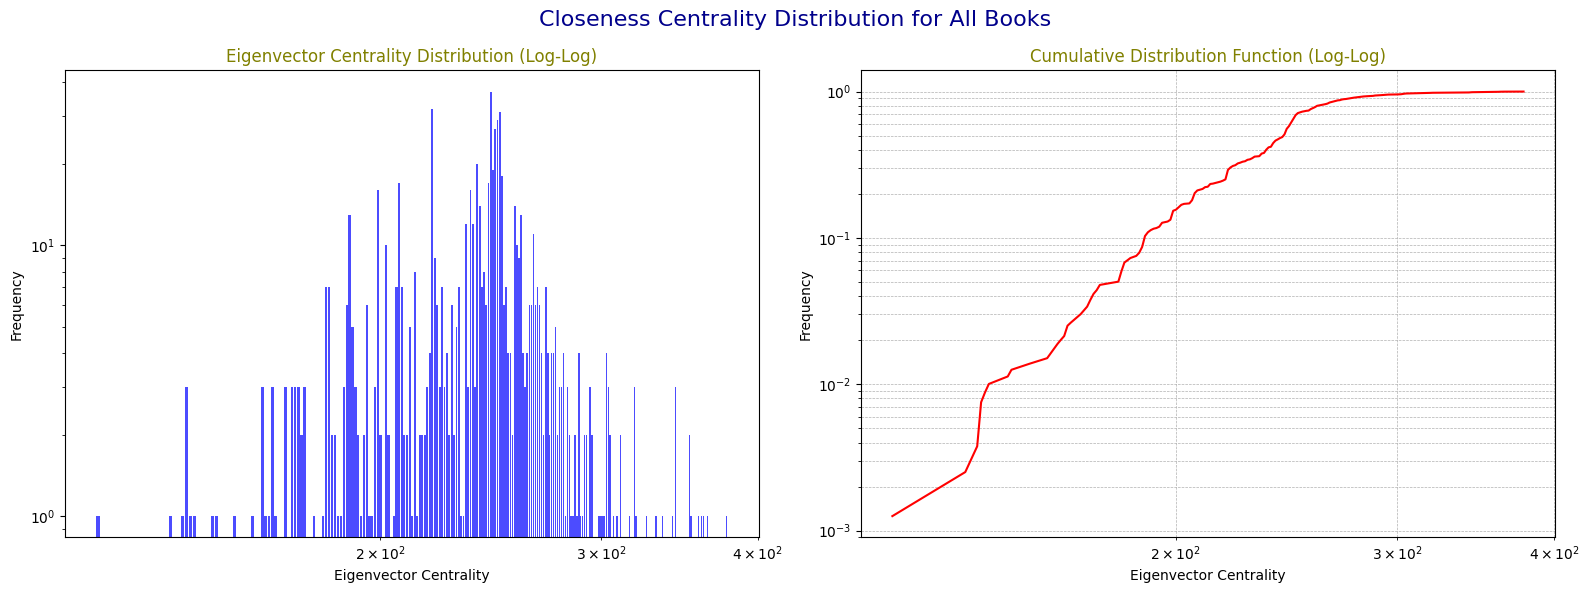
\includegraphics[width=0.7\textwidth]{closeness-distrib-all-books.png}
		\caption{Closeness Centrality Distribution for All Books}
		\label{fig:closeness-distrib}
	\end{figure}
	
	\subsection*{Betweenness Centrality}
	
	Betweenness centrality highlights the key narrative role of broker characters—those who connect distant parts of the story. In Book 1, most characters have near-zero values, but a few figures like Tyrion, Cersei, Varys, and Littlefinger stand out for linking otherwise disconnected subplots.
	
	As the series progresses, the distribution evolves: Book 2 sees new intermediaries like Brienne and Davos emerge due to the fragmented fronts of the War of the Five Kings. Book 3 has the widest tail, as events like the Red Wedding create many narrative bottlenecks and raise the brokerage role of secondary characters. Book 4 shows a contraction, with few central figures tying together largely separate storylines across distant regions. In Book 5, the tail expands again—characters like Jon, Tyrion, and Barristan help reconnect dispersed clusters.
	
	In the combined network, the distribution follows a power-law: most characters have negligible betweenness, while a small elite holds structural control. Compared to other centrality measures, betweenness is the most unequal—over 70\% of nodes have minimal scores, and fewer than 5\% exceed double digits. Shifts in this metric often align with narrative events like the removal or rise of key brokers, underlining their central role in maintaining story cohesion.
	
	\begin{figure}[htbp]
		\centering
		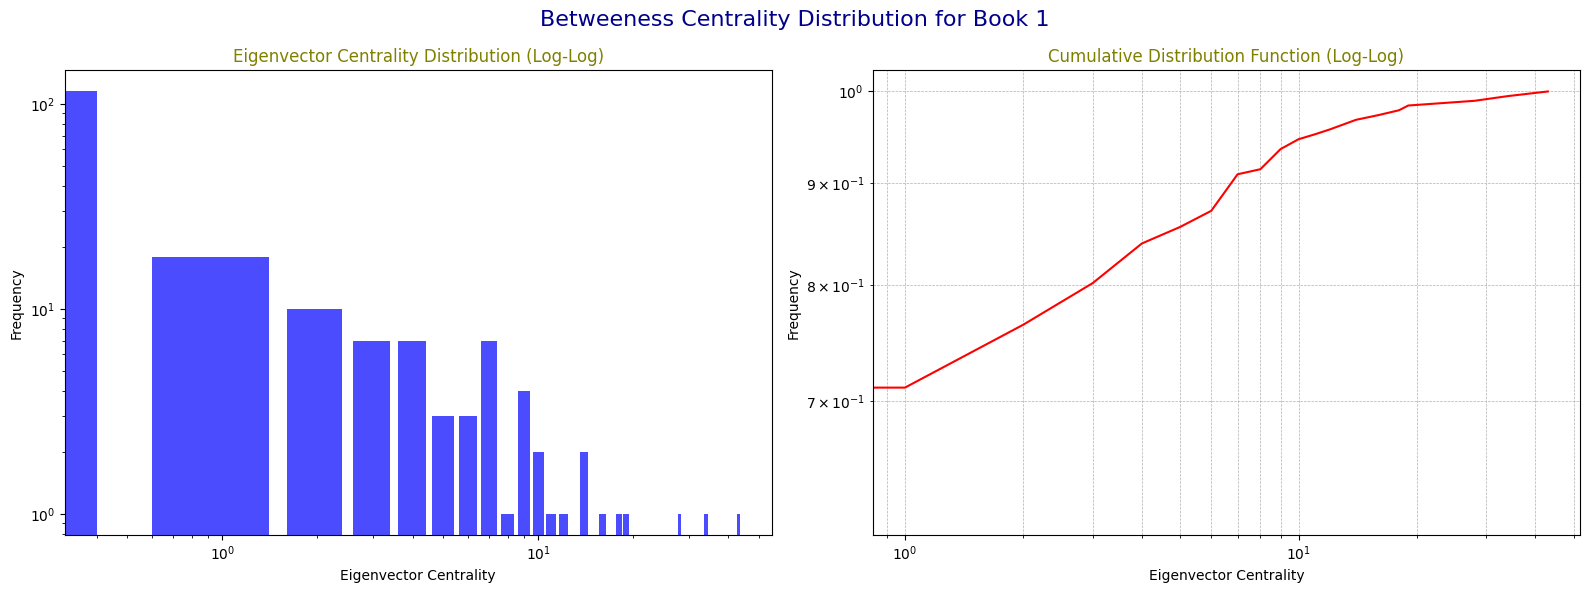
\includegraphics[width=0.7\textwidth]{betweenness-distrib-book1.png}
		\caption{Betweenness Centrality Distribution for Book 1.}
		\label{fig:betweennessbook1}
	\end{figure}
      \FloatBarrier
	\subsection*{Local Clustering Coefficient}
	The scatterplots that compare the average local clustering coefficient 
	with degree centrality show a clear increase in every single book and in the combined network.
	
	Characters with many interactions also belong to very close neighbourhoods whose members
	are highly connected to each other, so the coefficient quickly rises toward one for medium
	to high degrees and then levels off. In contrast, characters on the edge of the story 
	have only a few links and much lower clustering, which means they appear in sparse or 
	short-lived contexts. This result matches the way the plot is organised. 
	
	The narrative moves across several separate locations such as Winterfell, King's Landing, 
	the Wall, and Essos, each with a fairly stable group of characters who mainly talk among 
	themselves.
	
	Within each location the social network is almost a clique, 
	so once a character becomes central there, the chance that any 
	two of their contacts have also interacted is close to certain. 
	This explains the flat top of the curves.
	The different steepness at the beginning of the curves reflects the shifting narrative focus.
	Books that emphasise court politics, especially Books 2 and 3, 
	have steeper slopes because the royal court is an exceptionally 
	dense conversational hub, while Book 4, which spreads attention over more places, 
	has a gentler rise. 
	
	Overall, the plots show that being a popular character is not only a personal trait but also a feature that emerges inside cohesive local communities whose members often appear together and exchange dialogue.
	
	\begin{figure}[htbp]
		\centering
		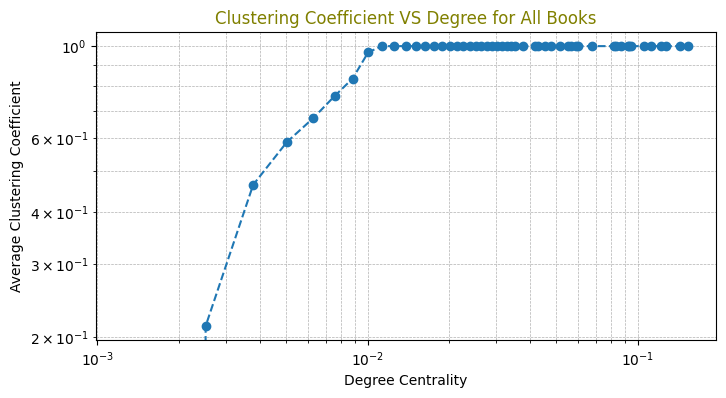
\includegraphics[width=0.7\textwidth]{local_clust_all_books.png}
		\label{fig:localclustcoeff}
		\caption{
			Log log plot of average clustering versus degree. Nodes with few links show low clustering, while highly connected nodes approach a clustering value of one.            }
	\end{figure}
	\FloatBarrier
	\subsection*{Global Network Metrics}
	We examined several global network metrics to understand the overall structure of the character interaction networks.
	Network {density}, the fraction of actual to possible connections, is initially 0.039 in Book 1, reflecting the early narrative focus on the Stark family. Density decreases in subsequent books and drops below one percent for the combined five-book network, as the character roster expands more rapidly than their interactions.
	The {connectedness} index is consistently one for all individual books and the combined network, indicating that a path exists between any two characters in the graph.
	{Compactness} remains low across all books (ranging from 0.193 to 0.150, with the combined network at 0.160), which aligns with the narrative's geographic dispersion and the presence of many intermediaries separating characters.
	{Transitivity}, measuring the prevalence of character triangles, declines from 0.33 in Book 1 to 0.20 in Book 5 (settling near 0.21 for the combined network). This trend further confirms the increasing geographic spread and fragmentation of the story.
	
	\subsection*{Centralisation and Core-periphery Indices}
	Centralisation measures the dominance of a few characters. Degree centralisation is highest in Book 1 (approx. 0.32). Betweenness centralisation notably increases from Book 1 (48) to Book 5 (>140), indicating that a small elite gains more control over information flow on critical story bridges in later books.

	Core-periphery analysis supports this. Degree-based analysis shows Book 1 has a compact core and a sparse periphery. While the optimal core size grows with the cast, the periphery remains proportionally large, with most characters at the margins. K-core decomposition sharpens this: Book 1's 11-core contains 23 resilient nodes. By Book 5, the densest core is a 6-core of only 17 characters, with about 300 in the periphery.
      So, a small set of pivotal figures consistently maintains network cohesion and channels information flow across its diverse regions.
	
	\section{Conclusion}
	\label{conclusion}
	
	This project mapped and analyzed the social network of characters in *A Song of Ice and Fire*, finding that network analysis illuminates the story's complex character dynamics. Constructing a co-occurrence network for the five books allowed us to identify key characters and their evolving roles.

	Centrality measures consistently identified influential figures and revealed insights, such as Stannis Baratheon's unexpected high betweenness centrality, suggesting his role as a crucial bridge despite fewer connections. Similarly, characters like Varys and Petyr Baelish stood out for linking separate groups.

	Clique detection and k-core decomposition showed that network-identified groups often corresponded to formal story groups (house, location, alliance). In later books, highest-order k-cores isolated clusters like the King's Landing court or the Night's Watch enclave, mirroring the narrative's split into concurrent storylines.

	Global metrics further described this social world. The network's disassortativity (hubs connecting to peripheral characters) produces a star-like hierarchy. A clear small-world effect was also evident: locally clustered groups are connected by bridge characters, ensuring short average path lengths, reflecting a world with distinct yet interconnected regions and plots.

	Overall, the strong correspondence between quantitative results and the novel's narrative structure suggests our network-based approach captured meaningful aspects of character importance and relationships.

	In summary, this work demonstrates the value of applying social network analysis to literature. Numerical metrics validated and enriched understanding of this complex story by confirming central characters, ranking importance, tracing role evolution, and uncovering communities and bridging roles, complementing traditional literary analysis with an evidence-based view of story architecture. The study's significance lies in its interdisciplinary approach, connecting computational methods with narrative analysis to illuminate *Game of Thrones*' structure. Quantifying interactions reinforced intuitions about heroes and factions and offered new perspectives on the plot's social structure, suggesting network science as a promising tool for exploring fictional social networks in other large narratives.

	Future studies could build on this by refining network construction (e.g., distinguishing interaction types, weighting connections) and comparing book-based networks to other representations (e.g., the television adaptation).
	
	\section{Critique}
	Our work substantially addressed the primary goal: identifying and measuring character importance in a complex, multi-plotline narrative. Social network metrics successfully identified principal characters across books, aligning with expected protagonists, and quantified their evolving importance through connectivity, influence, and brokerage roles.

	However, limitations exist. Network centrality, our primary measure (i.e., connectivity in the co-occurrence graph), highlighted narrative influence but might overlook characters crucial via subtle or behind-the-scenes actions. Indeed, some key figures didn't top all metrics, indicating our method captures social connectivity but not all facets of importance (e.g., psychological, thematic).

	Furthermore, results depended on the co-occurrence network dataset, an approximation of true interactions. This method can link merely co-mentioned characters and treats all interactions equally. These simplifications mean that while providing a strong structural analysis, our project addressed the research problem significantly but omitted some storytelling subtleties uncapturable by a purely network-based method.

	Future improvements could involve: 
	\begin{enumerate}
	    \item {Data Refinement:} Using advanced NLP for more accurate interaction identification (e.g., dialogue vs. co-mention, interaction type) and contextual data (chapter, location) to filter noise; incorporating TV show data or appendices could also offer verification.
	    \item {Alternative Modeling:} Employing temporal/dynamic network models for continuous importance tracking, or multiplex networks for richer social complexity by distinguishing relationship types (family, alliance).
	    \item {New Metrics/Techniques:} Analyzing network resilience via simulated character removal, using community detection algorithms for faction identification, and correlating network importance with external measures (e.g., POV chapters, fan polls).
	\end{enumerate}

	In summary, our project significantly advanced the understanding of character importance and structural patterns in Game of Thrones using Network Analysis, confirming key characters and network features. However, it only partially captured the full richness of character importance. Future work with refined data, models, and metrics could address remaining gaps, enhancing the bridge between quantitative network science and qualitative literary analysis.
\end{document}

